\documentclass{article}
\usepackage[a4paper, margin=3cm]{geometry}
\usepackage{graphicx}
\usepackage{algorithm}
\usepackage{algpseudocode}
\usepackage{hyperref}
\usepackage{comment}
\usepackage{amsmath}
\usepackage{enumitem}
\usepackage{amsfonts}
\usepackage{tikz}
\usetikzlibrary{arrows.meta,positioning,fit,calc}
\usepackage{rotating}

\newtheorem{theorem}{Theorem}[section]   % numbered per section
\newtheorem{lemma}[theorem]{Lemma}       % shares numbering with theorem
\newtheorem{corollary}[theorem]{Corollary}
\newtheorem{definition}[theorem]{Definition}
\usepackage{titling}

% Title formatting
\pretitle{\centering\huge\bfseries\vspace{4em}}
\posttitle{\par\vspace{2em}}

\preauthor{\centering\large}
\postauthor{\par\vspace{1em}}

\predate{\centering\small}
\postdate{\par\vspace{6em}}


\setlength{\parindent}{0pt} % no indend automatically everywhere

\title{Project Report\\Binary Heap and Dijkstra's Algorithm}
\author{
	\centering
	Josefine Lindmar
	Sonja Joost
}
\date{\today} % empty date

\begin{document}

\maketitle

\begin{center}
    \section*{Introduction}
\end{center}
This report presents a Lean formalization of a verified binary heap and a correctness development for Dijkstra's shortest-path algorithm that uses the heap as its priority queue. The heap part adopts a tree-based representation and implements the core operations (`heapify`, `insert`, `extract\_min`, `decrease\_key`), together with correctness proofs that these operations preserve the heap invariant, maintain membership and size properties, and satisfy behavioral laws required by Dijkstra's algorithm. These verified properties form a clean priority-queue abstraction that the algorithmic layer relies on. The Dijkstra development implements neighbor relaxation as a fold and the recursive driver `dijkstra\_rec`, and proves a number of lemmas used in the standard correctness argument; these are combined via a minimal-counterexample proof to establish the algorithm's correctness.
\newpage
\section{Binary Heap}
\textbf{Goal.} The goal of the binary heap part of the project is to formalize the binary heap together with the operations needed for the Dijkstra algorithm. This included the following:
\begin{itemize}
    \item \texttt{heapify}: Establish the heap invariant for a binary tree whose children are min heaps, furthermore used as subroutines for several operations
    \item \texttt{insert}: Add a new key to the heap and restore the binary heap invariant by bubbling the element to its correct position.
    \item \texttt{extract-min (/max)}: Pop the minimum (resp. maximum) element from the heap and restore the binary heap invariant by placing a leaf node at the root and trickling it down to the position it belongs to.
    \item \texttt{decrease-key (/increase-key)}: Decrease (resp. increase) the value of a  key to the new value, which is assumed to be less than or equal to the current key's value, and restore the heap invariant so that the node is at the correct position according to its new value.
\end{itemize}

\subsection*{Data Structure}

A binary heap is a data structure that represents data as a nearly complete binary tree \cite{clrs}. The binary heap must satisfy the heap condition, which depends on the type of heap. There are min and max heaps, where the root is the smallest or highest value, respectively. In a min heap, the value of each node is less than or equal to its parent's value. In a max heap, the value of each node is greater than or equal to its parent's value. In this project, we formalized the min heap.


A binary heap as two possible representations. It can be viewed as a binary tree as well as an array that is structured as a binary tree through the indices. As the binary tree representation allows for the straightforward possibility of performing structural induction, we chose to take a binary heap as the underlying data structure for the binary heap.
\newline

\small
\texttt{inductive BinaryTree (}\(\alpha\)\texttt{ : Type)}\\
\texttt{| leaf : BinaryTree }\(\alpha\)\\
\texttt{| node : BinaryTree }\(\alpha\)\texttt{ $\to$ }\(\alpha\)\texttt{ $\to$ BinaryTree }\(\alpha\)\texttt{ $\to$ BinaryTree }\(\alpha\)
\\\,\\
We chose to allow the binary heap to be of any type $\alpha$. As we shall later see, there are some restrictions on $\alpha$ needed for the implementation of some operations. The values of the nodes are assigned by a function $f$ that is passed along with the binary tree. $f$ assigns to each node a value of type \texttt{ENat}. \texttt{ENat} allows for the representation of infinity which is needed for the Dijkstra algorithm.
The binary min heap invariant is then defined as a proposition on the binary tree that holds whenever all nodes have a smaller value assigned to by $f$ than its parents:
 \newline
 
\texttt{def is\_min\_heap : BinaryTree }$\alpha$\texttt{ → (ordering : }$\alpha$\texttt{ → ENat) → Prop}\\
\texttt{| leaf, \_ => true}\\
\texttt{| node l v r, f => match l, r with}\\
\texttt{| leaf, leaf => true}\\
\hspace*{10mm}\texttt{| node \_ lv \_, leaf => f v }$\le $\texttt{ f lv }$\wedge$\texttt{ is\_min\_heap l f}\\
\hspace*{10mm}\texttt{| leaf, node \_ rv \_ => f v }$ \le $\texttt{ f rv }$\wedge$\texttt{ is\_min\_heap r f}\\
\hspace*{10mm}\texttt{| node \_ lv \_, node \_ rv \_ =>}\\
\hspace*{20mm}\texttt{ f v } $\le $\texttt{ f lv }$\wedge$\texttt{ is\_min\_heap l f }$\wedge$\texttt{}
\texttt{ f v }$ \le$ \texttt{ f rv }$\wedge$\texttt{ is\_min\_heap r f}\\

\subsection{Operations}
For the operations on the binary heap, we show that they function as expected. In particular, we show that the functionality is correct and that the binary heap invariant is established (or preserved, respectively).
\subsubsection{heapify}
Heapify is a subroutine that is used by several of the operations mentioned in the following. It takes a binary tree as input for which the heap invariant holds for both of its children, if they exist, and moves the root node to the correct position so that the heap invariant holds for the whole binary tree. We show in the formalization that it establishes the heap invariant and that the output contains the exact same nodes as the input. We formulate the theorem to apply to general trees (as opposed to only nodes that have children) to enable induction in the proof. In particular:
\\

\begin{theorem}[Theorem. Correctness \texttt{heapify}.]
Let $bt$ be a binary tree over elements of type $\alpha$, and let $f: \alpha \to \mathbb{N} \cup \{\infty\}$ be a function. Then:
 \begin{align}  
&(\forall v. v \in bt \iff v \in \texttt{heapify}(bt, f)) \;\land \\
&(\exists l, v, r. bt = \texttt{node} (l, v, r) \Rightarrow \texttt{is\_min\_heap}(l, f) \land \texttt{is\_min\_heap}(r, f) \Rightarrow  \texttt{is\_min\_heap}(\texttt{heapify}(bt, f), f))
 \end{align}
\end{theorem}

\textbf{English explanation.} To prove the first part, we just show that no node was added or removed during the heapify operation. 

The second part requires a proof by functional induction over \texttt{heapify}. The base cases are trivial, as the \texttt{leaf} and the node with only \texttt{leaves} as children satisfy the heap invariant by definition. The cases that do not call \texttt{heapify} recursively can be solved with the definition and the assumptions available at the respective proof states. For the other three cases, the structure of the proof is similar: We use the fact that a binary tree satisfies the heap condition if both children are min heaps and the value assigned to the root node is less than or equal to that of the children. This allows us to use the induction hypothesis for the two children, and we can use the conditions for the cases to show that the root indeed holds the minimum value.\\


\textbf{Lean correspondence.}
We prove both statements separately. We split the first into both directions (\texttt{contains\_then\_heapify\_contains, heapify\_contains\_then\_contains}) and can prove both with functional induction over \texttt{heapify} and the definition of \texttt{contains} (which corresponds to $\in$).
We do \texttt{fun\_induction heapify generalizing l r v; all\_goals expose\_names}. Note that we need to generalize the induction hypothesis in order to apply it to the children of the tree. For the leaf cases and the ones that do not recurs, we can simply use the definition of heapify together with the assumptions. For the cases that call \texttt{heapify}, we define a helper lemma that shows that if the two children are min heaps and the value assigned to the root is less than or equal to that of the children, then the tree is a min heap (\texttt{left\_and\_right\_are\_min\_heap\_and\_root\_is\_min\_of\_children\_is\_min\_heap}). To show that the children are min heaps we can simply use the induction hypothesis (since the children are min heaps, their children are also min heaps, so the induction hypothesis can be applied (by \texttt{min\_heap\_then\_left\_and\_right\_are\_min\_heap}) and the assumptions. To show that the root value is smaller that the values of the children, we use the fact, that in the \texttt{heapify} we switch the root with the smaller child if it is larger and then the smallest value of each of the children is smaller than the root because the children are min heaps (\texttt{root\_is\_min\_of\_children, min\_heap\_member\_le\_root}) and its members did not change except for the potentially switched root whose value is larger (\texttt{heapify\_contains\_then\_contains}).

\subsubsection{insert}
For the \texttt{insert} operation, we show that all members are equal with the addition of the inserted node.
\\
\begin{theorem}[Insert Correctness]
Let $bt : \mathsf{BinaryTree}\,\alpha$ and $f : \alpha \to \mathbb{N} \cup \{\infty\}$. Then
\begin{align}
\bigl(
\forall v\, v',\;
 v \in bt\; \lor v = v'
\;\Longleftrightarrow\;
v \in (\mathsf{insert}\; bt\; v'\; f)\;
\bigr)
\;\land\;\\
\bigl(
\mathsf{is\_min\_heap}\; bt\; f
\;\Longrightarrow\;
\mathsf{is\_min\_heap}\; (\mathsf{insert}\; bt\; v\; f)\; f
\bigr).
\end{align}
\end{theorem}

\textbf{English explanation.}
For the correctness proof, we show two parts. The first, membership preservation,  can be further decomposed into the two directions. Showing that the tree with the inserted node still contains all nodes can be shown via functional induction over the insert assuming that there is a node $vi$ n $bt$. The base case is trivial. If the binary tree is initially a leaf, then the case can be solved by contradiction as a leaf cannot contain a value. In the step case, we assume that v is contained in the current node and analyze whether it is at the root or in one of the sub trees. If it is in a sub tree, we apply the induction hypothesis to that sub tree and then reconstruct the proof for the inserted tree, showing that insertion preserves membership of existing elements. To show that the inserted node is in the new tree, we can again perform simple function induction. If the tree was a leaf, the value is added as the root. In the other case, it either is inserted at the root, which concludes the proof, or it is propagated to the children. In that case, we can use the induction hypothesis.
In the other direction, we can again perform functional induction over the insert. The leaf case is trivial, in that case $v = v'$. In the two step cases, we make a case distinction over the membership of $v$. It is either at the root, in which case we have $v=v'$, or it is a member of the children. In that case, we can use the induction hypothesis.

In the second part of the proof we show that insertion maintains the min-heap invariant, assuming that the original tree is a min-heap. We use functional induction over the insert. The base case is trivial as any node with only leafs as children is a min heap by definition. For the two step cases, we again make use of the fact that if the children are min heaps and their roots are smaller than the root of $bt$, then $bt$ is a min heap. As the condition in the definition ensures that the value is inserted at the root if it is smaller than the current node, we can show that the root remains the minimum. Since the node is propagated to the children if it is larger, we can make use of the induction hypothesis.\\

\textbf{Lean correspondence.}
We use a structure similar to that described above. We show the first part with the lemmas \texttt{insert\_contains\_inserted} and \texttt{contains\_then\_insert\_contains} for one direction and \texttt{insert\_- contains\_then\_contains\_or\_inserted} for the other, respectively. All are shown with functional induction on the \texttt{insert}.

The preservation of the heap invariant is shown in the lemma \texttt{insert\_preserves\_min\_heap}. It makes use of \texttt{left- \_and\_right\_are\_min\_heap\_and\_root\_is\_min\_of\_children\_is\_min\_heap} and  \texttt{min\_heap\_then\_left\_and\_right- \_are\_min\_heap} which shows that the children of a min heap are min heaps if they exist.

\subsubsection{extract\_min}

For the \texttt{extract\_min} operation, we show that removing the minimum element preserves all remaining elements and maintains the min-heap invariant. Additionally, we show that the extracted element corresponds to the minimum priority stored in the heap. The \texttt{extract\_min} operation returns a pair: the left part is the minimal element, and the right part is the tree with the element removed.

\begin{theorem}[Extract-Min Correctness]
Let $bt, l, r : \mathsf{BinaryTree}\,\alpha$, $v, v' : \alpha$, and
$f : \alpha \to \mathbb{N} \cup \{\infty\}$. Then
\begin{align}
&\bigl(
\mathsf{contains}\; (\mathsf{extract\_min}\; bt\; f).2\; v
\;\Longrightarrow\;
\mathsf{contains}\; bt\; v
\bigr)
\;\land\;\\
&\bigl(
bt = \mathsf{node}\; l\; v\; r
\;\Longrightarrow\;
\mathsf{contains}\; bt\; v'
\;\Longrightarrow\;
v \neq v'
\;\Longrightarrow\;
\mathsf{contains}\; (\mathsf{extract\_min}\; bt\; f).2\; v'
\bigr)
\;\land\;\\
&\bigl(
bt = \mathsf{node}\; l\; v\; r
\;\Longrightarrow\;
\mathsf{is\_min\_heap}\; bt\; f
\;\Longrightarrow\;
\exists bt'\, v',\;
\mathsf{extract\_min}\; bt\; f = (\mathsf{some}\; v', bt')
\;\\ &\land\;
\mathsf{is\_min\_heap}\; bt'\; f
\;\land\;
f\,v = \mathsf{heap\_min}\; bt\; f
\bigr).
\end{align}
\end{theorem}

\textbf{English explanation.}
The correctness proof of \texttt{extract\_min} consists of several interconnected parts.

Firstly, we show that every element contained in the resulting tree after extraction was already present in the original tree. This establishes that \texttt{extract\_min} does not introduce any new elements. The proof proceeds by structural reasoning about the definition of \texttt{extract\_min}. Since the operation only removes the root element and restructures the remaining tree, all elements in the resulting tree must have originated from the original heap.
Moreover, we show that extraction preserves the membership of all elements except the removed root. If the original tree is a node with the root value $v$, the resulting tree will have all the elements except $v$. Both can be shown via functional induction on the definition and by case distinction if the element contained is the root or not.

Secondly, assuming that the original tree satisfies the min heap invariant, we show that \texttt{extract\_min} returns a value $v'$ together with a tree $bt'$ and the resulting tree $bt'$ is again a min heap and the extracted value $v'$ corresponds to the minimum priority stored in the original heap. This follows from the definition of \texttt{extract\_min}, which removes the root of the heap and then restores the heap property by rearranging the remaining nodes. The induction hypothesis ensures that all recursive calls preserve the heap invariant.
\\
\textbf{Lean correspondence.}

In Lean, we followed a similar structure as described above: We defined the auxiliary lemmas 
\texttt{extract\_min- \_correct\_node},
\texttt{extract\_min\_contains\_then\_contains}, and
\texttt{contains\_then\_extract\_min\_contains\_except- \_root}, each of which proves one piece of the theorem. To implement the \texttt{extract\_min} function, we defined a \texttt{get\_last} function that finds the last element. \texttt{extract\_min} then puts it at the root position instead of the minimum element, which is removed from the tree and returned. \texttt{extract\_min} applies the \texttt{heapify} function to restore the heap invariant. 
Due to this setup, we first showed membership lemmas for \texttt{get\_last} and then used them in the proofs for \texttt{extract\_min}.
For the proof of the heap invariant, we showed that if $bt$ is a min heap, then, for the result of  \texttt{get\_last} holds that the left aud right sub trees are min heaps (\texttt{min\_heap\_then\_left\_and\_right\_are\_min\_heap}). This is the precondition to show that \texttt{heapify} restores the heap invariant.  
The proof leverages these decomposition/re-composition lemmas like \texttt{min\_heap\_then\_left\_and\_right\_are\_min\_heap} and \texttt{left\_and\_right\_are\_min\_heap\_and\_root\_is\_min\_of\_child- ren\_is\_min\_heap} to move between global heap facts and local child facts to avoid unfolding the inductive definition of \texttt{is\_min\_heap}.

\subsubsection{decrease\_priority}

For the \texttt{decrease\_priority} operation, we show that all existing members of the binary tree are preserved and that the min-heap invariant is maintained when the priority of a node is decreased. Note that we need a precondition to hold for $\alpha$: it must be decidable whether elements of this type are equal to each other.
\begin{theorem}[Decrease Priority Correctness]
Let $bt : \mathsf{BinaryTree}\,\alpha$, $v, v' : \alpha$, and $f : \alpha \to \mathbb{N} \cup \{\infty\}$, assuming decidable equality on $\alpha$. Then
\begin{align}
&\mathsf{contains}\; bt\; v
\;\Longleftrightarrow\;
\mathsf{contains}\; (\mathsf{decrease\_priority}\; bt\; v'\; f)\; v
\;\land\;
\\&\bigl(
\mathsf{is\_min\_heap}\; bt\; f
\;\Longrightarrow\;
\mathsf{is\_min\_heap}\; (\mathsf{decrease\_priority}\; bt\; v\; f)\; f
\bigr).
\end{align}
\end{theorem}

\textbf{English explanation.}
The proof of the correctness for \texttt{decrease\_priority} consists of two parts. Firstly, we show that decreasing the priority of a node does not change the set of elements contained in the tree. This is split into two parts and is shown by induction on the definition of \texttt{decrease\_priority} , which is a combination of first removing and then inserting the node into the tree. We show that executing them in sequence leads to the same members in the tree. 
Secondly, we show that the min heap invariant is preserved when decreasing a key. As \texttt{decrease\_priority} uses heapify, this is shown by the proof of the correctness of heapify.\\

\textbf{Lean correspondence.}
 The proof proceeds by a small case split on whether the element is a member of \texttt{bt}: if the element is present, the implementation performs remove followed by insert, otherwise it is a no-op. The lemma \texttt{contains\_then\_decrease\_priority\_contains} shows that any element of the original tree remains present after \texttt{decrease\_priority}, and it is proven by structural induction on \texttt{decrease\_priority} (and by delegating to containment lemmas for \texttt{remove} and \texttt{insert}). The lemma \texttt{decrease\_priority\_contains\_then\_contains} proves the converse direction, that any element found after the operation already belonged to the original tree; this uses shape facts about \texttt{insert} and \texttt{remove}. The preservation of the heap property is established in \texttt{decrease\_priority\_preserves\_min\_heap}, which is explained by the two cases: the no-op case is trivial, and the present-element case comprises \texttt{remove\_preserves- \_min\_heap} and \texttt{insert\_preserves\_min\_heap} to show that the final tree remains the heap minimum. Crucial auxiliary lemmas used in these arguments include \texttt{remove\_preserves\_members\_except\_v} (so removing does not accidentally drop unrelated members), \texttt{insert\_contains} and \texttt{insert\_contains\_then\_contains\_or\_inser- ted} (to reason about the newly inserted element versus \ existing ones), and the shape lemma \texttt{insert\_is\_node} that enables case analysis on constructed nodes. The proof strategy is therefore to reduce the correctness of \texttt{decrease\_priority} to the correctness of \texttt{remove} and \texttt{insert}. Combining these lemmas yields the final equivalence and the heap-preservation properties, completing the proof of \texttt{decrease\_priority\_correctness}.

\subsection{Summary}
This section provides an overview of the formalization work on the Binary Heap and outlines the remaining proof obligations.\\

\textbf{Completed work.} Our formalization of the Binary Heap is composed of the data structure together with its invariant to ensure that the binary tree is indeed a min heap and the operations on it. Among the results established are: 
\begin{itemize}
  \item formalization of the min heap invariant on the binary tree
  \item formalization of the core operations performed on the heap \texttt{heapify, insert, extract-min, decrease- priority}
  \item proofs of heap invariant preservation of the operations and the auxiliary operations
  \item proof of membership preservation to prove only necessary elements were added/removed 
  \item proofs of correctness combining the heap preservation and membership preservation properties
  \item providing a binary heap interface for Dijkstra's shortest path algorithm including additional helper lemmas including size and structural invariants
\end{itemize}


\textbf{Potential further steps.} Possible next steps would be to transfer the tree-based implementation to an array-based one. This will allow for the precise implementation of the operation's algorithm and performing runtime analysis on them. As most of the proofs were shown by functional induction, it can be assumed that they can be reused to some extent.
\newpage

\section{Dijkstra's algorithm}
\paragraph{Goal.} Our goal was to formalize Dijkstra's algorithm \cite{dijkstra} over finite (connected) graphs and prove correctness, using a priority queue abstraction.\\

\paragraph{Solution.} We represent the graph as a finite simple graph \cite{mathlib4} so that vertices have decidable equality (exactly as we have seen in the BinarySort examples in class). Distances use extended natural numbers (so an unknown distance can be “infinity”), called \texttt{ENat} in Lean. The algorithm state is just a pair: a distance map from vertices to these extended naturals (\(\texttt{dist} : V \to \mathbb{N}_\infty\)) and a binary-heap priority queue (\(\texttt{queue} : \texttt{BinaryHeap} \, V\)). The heap that was implemented in the first part of the project exposes abstract operations (empty check, extract-min, decrease-priority, etc) and the proof for the algorithm only relies on their contracts. 

\subsection{Implementation}

The implementation of the algorithm is split up into three parts: 
\begin{itemize}
	\item Relaxation (Lean: \texttt{relax\_neighbors}) is a simple loop over the neighbors of a vertex u that updates each neighbor v by setting $dist(v)$ to the minimum of its current value and $dist(u)+1$, and it updates the queue (implemented as BinaryHeap) accordingly.
	\item The recursive core of Dijkstra (Lean: \texttt{dijkstra\_rec}) repeatedly extracts the current minimum u, relaxes u’s neighbors (updating the distance map and heap), and then recurses on the new state.
	\item The top-level function (Lean: \texttt{dijkstra}) initializes distances with 0 at the source and infinity elsewhere, inserts the source into the heap, and starts the recursion.
\end{itemize}



\subsection{Termination}
\label{termination}
We split the implementation into three parts: \texttt{dijkstra} (a non-recursive wrapper), \texttt{dijkstra\_rec} (the recursive core), and \texttt{relax\_neighbors} (implemented as a fold over the finite list of neighbors). Since we only need to prove termination for recursive definitions, we only have to show termination explicitly for \texttt{dijkstra\_rec}.

We prove termination by the measure \texttt{queue.sizeOf}: 
We prove that the heap measure strictly decreases, i.e. $\texttt{queue''.sizeOf} < \texttt{queue.sizeOf}$. Starting from a nonempty heap (the hypothesis $hq$ that $\texttt{queue} \neq \texttt{queue.empty}$ is used), the proof exposes the concrete definitions of the intermediate queues with $hq'\_eq$ and $hq''\_eq$ (both proven via reflexivity because queue' and queue'' are exactly the second components of extract\_min and relax\_neighbors respectively). The \texttt{calc} chain then rewrites \texttt{queue''.sizeOf} to \texttt{(relax\_neighbors g u dist queue').2.sizeOf}, applies the lemma \texttt{sizeOf\_relax\_neighbors\_le} to get a non‑strict inequality to \texttt{queue'.sizeOf}, rewrites \texttt{queue'.sizeOf} to the second component of \texttt{extract\_min}, and finally uses an exposed lemma from the BinaryHeap interface to get the strict decrease after extraction; together these steps yield the required strict decrease.\\


Besides the exposed lemma from the BinaryHeap interface, we also relied in this proof on the lemma \texttt{sizeOf\_relax\_neighbors\_le}. This lemma states that if we relax the neighbors using \texttt{relax\_neighbors} that the queue can only ever decrease in size. In Lean that is expressed as:
\begin{center}
    \texttt{BinaryHeap.sizeOf (Prod.snd (relax\_neighbors g u dist q)) $\le$ BinaryHeap.sizeOf q}
\end{center}
This lemma is important as it is used in total 4 times throughout our proofs. We can prove it using induction on the the neighbors of a node generalizing the distance map and priority queue. If the neighbors list is empty, the statement is obviously true (in Lean a simple \texttt{simp} is enough). If the neighbors are a list, however, we name dist' and queue' the result of applying the function f (the function applied to all entries in the fold) and show by case distinction that \texttt{queue'.sizeOf $\le$ q.sizeOf}. By applying the induction hypothesis on the tail we know that the size of BinaryHeap after the fold over the tail is \texttt{$\le$ queue'.sizeOf}. By chaining both equalities we can then finish the proof. 




\subsection{Correctness proof (\texorpdfstring{$\texttt{dijkstra\_correctness}$}{dijkstra\_correctness})}
Our goal is to prove that the algorithm is correct, i.e., for any vertex \(v\), the algorithm’s output equals the graph distance $\delta$ defined by Mathlib: \[(\texttt{dijkstra}\ g\ s\ v)\ v = \delta(g,s,v)\]

The proof proceeds by fixing the algorithm's output (concretely, set \( \texttt{dist} := \texttt{dijkstra}\ g\ s\ v \)) and deriving a contradiction from any alleged disagreement with the true graph distance. \\

We assume, for contradiction, that there exists a vertex \(u\) with \(\texttt{dist}\ u \ne \delta(s,u)\). Choose such a \(u\) that minimizes \(\delta(s,u)\), given by \texttt{minimal\_counterexample}. 
Note also that by \texttt{dijkstra\_source\_zero} the algorithm assigns \(0\) to the source, i.e. \(\texttt{dist}\,  s=0=\delta(s,s)\), so any counterexample cannot be the source. By the previous remark we have \(\delta(s,u)>0\), proven by the lemma \texttt{positive\_distance\_of\_counterexample}.

Take a shortest path from \(s\) to \(u\); this yields a predecessor \(y\) with \(y\sim u\) and
\[
\delta(s,u)=\delta(s,y)+1
\]
given by the lemma \texttt{exists\_pred\_on\_shortest\_path}.

Since \(\delta(s,y)<\delta(s,u)\), we have \[\texttt{dist}\ y=\delta(s,y)\] because $u$ was minimal.

Now apply the algorithmic per-edge final bound \texttt{relax\_adj\_final\_bound} to the edge \(y\sim u\). That lemma yields the upper bound
\[
\texttt{dist}\ u \le \texttt{dist}\ y + 1.
\]
Substituting \(\texttt{dist}\ y=\delta(s,y)\) and \(\delta(s,y)+1=\delta(s,u)\) gives \(\texttt{dist}\ u \le \delta(s,u)\).

We establish the global lower bound
\[
\forall u,\ \delta(s,u)\le \texttt{dist}\ u,
\]
provided by the lemma \texttt{never\_underestimates}. \\

The global and lower bound together force the equality \(\texttt{dist}\ u = \delta(s,u)\), contradicting the choice of \(u\) as a counterexample.
Hence no counterexample exists, and we conclude that \texttt{dijkstra\_correctness} is correct.\\


\textbf{Notes.} The development assumes the standard BinaryHeap contracts and constructs the correctness proof from a collection of named lemmas, many of which themselves rely on smaller auxiliary results. Figure~\ref{fig:dijkstra-deps} illustrates the dependency structure among the main lemmas used in the correctness proof of Dijkstra’s algorithm; for reasons of space and clarity, some minor lemmas are omitted from the diagram. All lemmas shown in the diagram have been fully formalized and proven, with only few exceptions. The lemma \\\texttt{exists\_extract\_or\_top} has not yet been completed. The lower-bound lemma \texttt{never\_underestimates} is not proven as it was assumed given / obvious in the original proof. In addition, two small helper lemmas that reason about the BinaryHeap (\texttt{extract\_min\_still\_correct\_1} and \texttt{extract\_min\_still\_correct\_2}) are left as \texttt{sorry}. Since these lemmas are not central to the core ideas presented in this report, we deliberately allocated our time to completing and refining the more essential proofs. The reasons these proofs remain unfinished are discussed in more detail in the corresponding sections on the following pages.

\begin{sidewaysfigure}
\centering
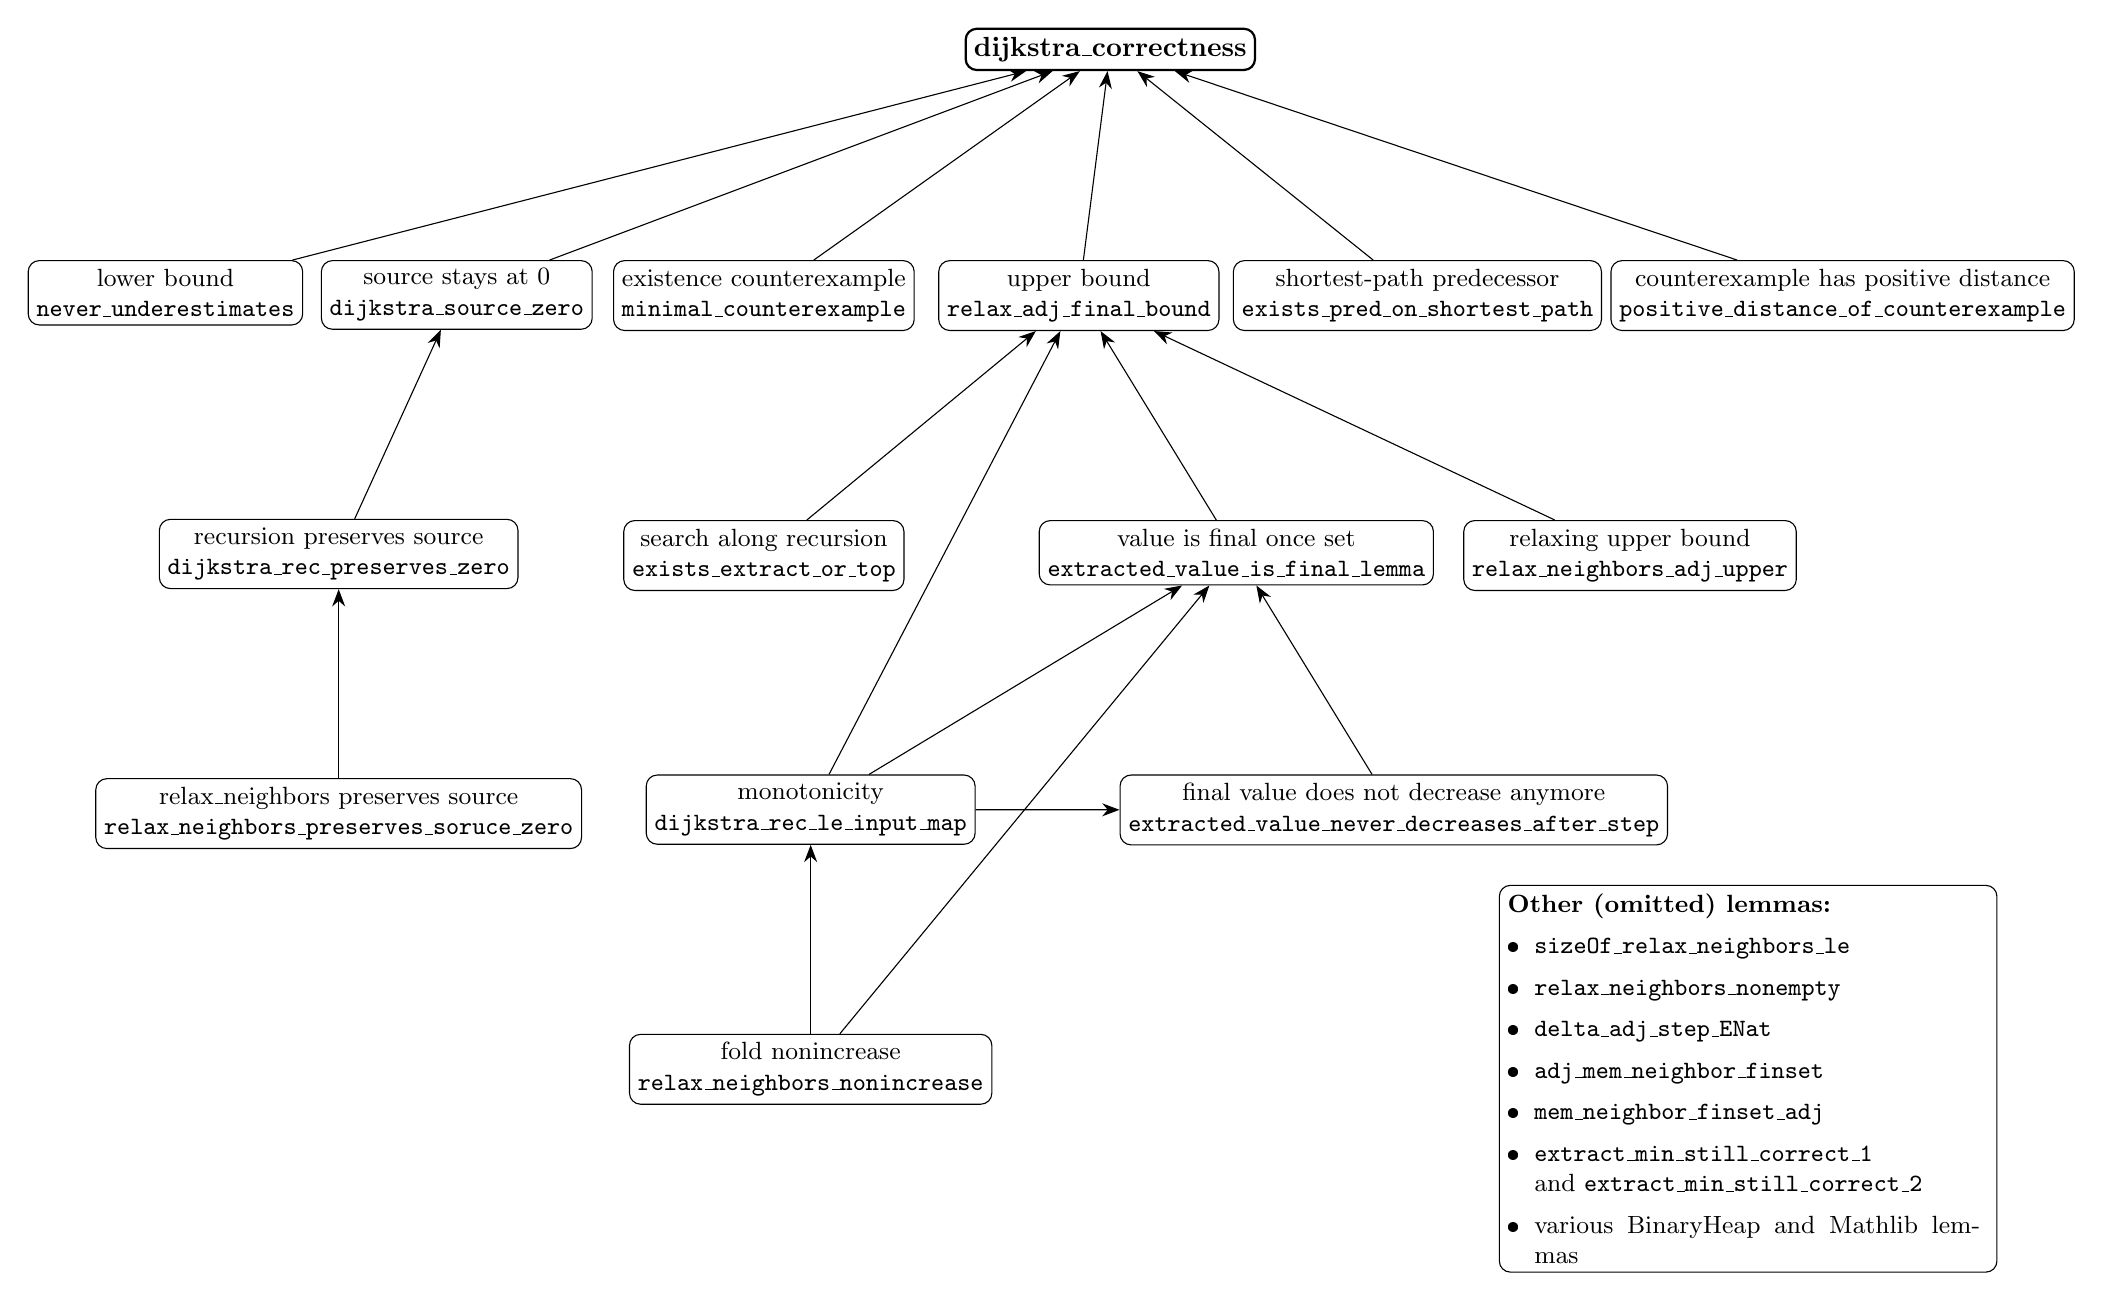
\begin{tikzpicture}[
  node distance=10mm and 12mm,
  box/.style={rectangle, draw, rounded corners, align=center, inner sep=3pt, font=\small},
  grp/.style={draw, rounded corners, inner sep=4pt, dashed},
  >={Stealth[length=2.2mm]},
  every edge/.style={draw, -{Stealth[length=2.2mm]}}
]
% Top layer: correctness
\node[box, font=\normalsize, thick] (CORR) {\textbf{dijkstra\_correctness}};

\node[box, below=24mm of CORR, xshift=-120mm] (LOWER) {lower bound\\\texttt{never\_underestimates}};
\node[box, below=24mm of CORR, xshift=-83mm] (ZERO_TOP) {source stays at 0\\\texttt{dijkstra\_source\_zero}};
\node[box, below=24mm of CORR, xshift=-44mm] (CNT) {existence counterexample\\\texttt{minimal\_counterexample}};
\node[box, below=24mm of CORR, xshift=-4mm] (EDGE) {upper bound\\\texttt{relax\_adj\_final\_bound}};
\node[box, below=24mm of CORR, xshift=39mm] (PRED) {shortest-path predecessor\\\texttt{exists\_pred\_on\_shortest\_path}};
\node[box, below=24mm of CORR, xshift=93mm] (CNT_DIST) {counterexample has positive distance\\\texttt{positive\_distance\_of\_counterexample}};

% Edges: correctness
\path (LOWER) edge (CORR);
\path (CNT) edge (CORR);
\path (ZERO_TOP) edge (CORR);
\path (CNT_DIST) edge (CORR);
\path (PRED) edge (CORR);
\path (EDGE) edge (CORR);

% LEVEL 2 (wider spacing to avoid horizontal overlap)
\node[box, below=24mm of EDGE, xshift=-40mm] (SEARCH) {search along recursion\\\texttt{exists\_extract\_or\_top}};
\node[box, below=24mm of EDGE, xshift=20mm]   (EVF)    {value is final once set \\\texttt{extracted\_value\_is\_final\_lemma}};
\node[box, below=24mm of EDGE, xshift=70mm]  (RAU)    {relaxing upper bound\\\texttt{relax\_neighbors\_adj\_upper}};
% Edges toward EDGE (per-edge final bound)
\path (SEARCH) edge (EDGE);
\path (EVF) edge (EDGE);
\path (RAU) edge (EDGE);

\node[box, below = 24mm of ZERO_TOP, xshift=-15mm] (ZERO_MIDDLE) {recursion preserves source\\\texttt{dijkstra\_rec\_preserves\_zero}};
\path (ZERO_MIDDLE) edge (ZERO_TOP);


% LEVEL 3
\node[box, below left=24mm and 8mm of EVF] (MONO) {monotonicity\\\texttt{dijkstra\_rec\_le\_input\_map}};
\node[box, below=24mm of EVF, xshift=20mm] (EVND) {final value does not decrease anymore\\\texttt{extracted\_value\_never\_decreases\_after\_step}};
\path (MONO) edge (EVF);
\path (MONO) edge (EDGE);
\path (MONO) edge (EVND);
\path (EVND) edge (EVF);

\node[box, below = 24mm of ZERO_MIDDLE] (ZERO_BOTTOM) {relax\_neighbors preserves source\\\texttt{relax\_neighbors\_preserves\_soruce\_zero}};
\path (ZERO_BOTTOM) edge (ZERO_MIDDLE);

% LEVEL 4
\node[box, below=24mm of MONO] (RNI) {fold nonincrease\\\texttt{relax\_neighbors\_nonincrease}};
\path (RNI) edge (MONO);
\path (RNI) edge (EVF);

% Node listing omitted/auxiliary lemmas
\node[box, below=5mm of EVND, xshift=45mm, align=left, font=\small] (OTHERS) {%
  \begin{minipage}{60mm}
  \textbf{Other (omitted) lemmas:}
  \begin{itemize}[leftmargin=*]
    \item \texttt{sizeOf\_relax\_neighbors\_le}
    \item \texttt{relax\_neighbors\_nonempty}
    \item \texttt{delta\_adj\_step\_ENat}
    \item \texttt{adj\_mem\_neighbor\_finset} 
    \item \texttt{mem\_neighbor\_finset\_adj}
    \item \texttt{extract\_min\_still\_correct\_1} \\and \texttt{extract\_min\_still\_correct\_2}
    \item various BinaryHeap and Mathlib lemmas
  \end{itemize}
  \end{minipage}
};

% Optional visual connector to indicate these are auxiliary to many nodes
%\path[dashed] (OTHERS.north) edge[bend left=30] (RNI.east);
%\path[dashed] (OTHERS.north) edge[bend left=20] (SEARCH.east);
%\path[dashed] (OTHERS.north) edge[bend right=10] (LOWER.east);

\end{tikzpicture}
\caption{Lemma dependency graph shaping the proof of correctness.}
\label{fig:dijkstra-deps}
\end{sidewaysfigure}

\newpage


\subsubsection{Lower bound (\texttt{never\_underestimates})}
\textbf{Statement.} For any vertex \(u\), Dijkstra's output never underestimates the true graph distance: \[(\texttt{dijkstra}\ g\ s\ t)\ u \ge \delta(g,s,u)\]

This lemma establishes a global lower bound on the algorithm's output. In the Lean file, this lemma is currently left as \texttt{admit}. All online references we found assume this property as a given, since it is so intuitive. We therefore treat this lemma as an axiomatic starting point for our correctness proof.

\subsubsection{Source preservation (\texttt{dijkstra\_source\_zero}, \texttt{dijkstra\_rec\_preserves\_zero}, \\
\texttt{relax\_neighbors\_preserves\_source\_zero})}
\textbf{Statement.} The source vertex \(s\) always maintains distance \(0\) throughout the algorithm: \[(\texttt{dijkstra}\ g\ s\ t)\ s = 0\]

\textbf{English explanation.} Dijkstra initializes \(\texttt{dist}(s) = 0\). We must show that this invariant is preserved through all recursive steps. The key observation is that \texttt{relax\_neighbors} only updates neighbors of the extracted vertex \(u\), and each update sets a neighbor's distance to \(\texttt{dist}(u)+1\). Since the graph is irreflexive, \(s\) is never a neighbor of itself, so it can only be updated if it appears as a neighbor of some other vertex \(u\). But even if \(s\) were a neighbor of \(u\), the update condition \(\texttt{dist}(u)+1 < \texttt{dist}(s)\) would require \(\texttt{dist}(u)+1 < 0\), which is impossible in extended naturals. Therefore, \(\texttt{dist}(s)\) remains unchanged at \(0\) after every relaxation step, and by induction on the depth of the recursion (using strong induction on the heap size), it stays \(0\) in the final output.\\

\textbf{Lean correspondence.} The proof is split into three lemmas in a bottom-up fashion. 
\begin{itemize}
    \item \texttt{relax\_neighbors\_preserves\_source\_zero} proves preservation for a single relaxation step. For that we first show that applying the update on a single neighbor will preserve the invariant (\texttt{step\_preserve}): If it is the source node, then relaxation is not possible, because no number plus 1 can be smaller than 0 in \texttt{ENat}. Otherwise, the result is immediate after a case distinction on if the neighbors (that are not the source) are relaxed or not. With induction on the neighbors we can show this for the entire fold (\texttt{fold\_preserve}). We can then easily close this goal with rewrites and \texttt{simpa}.
    
    \item Next, \texttt{dijkstra\_rec\_preserves\_zero} lifts this to the full recursion via strong induction on \texttt{sizeOf(queue)}: if the queue is empty the result is immediate; otherwise we combine the previous lemma to get \(\texttt{dist' source}=0\) after relaxation, then apply the induction hypothesis to the smaller post-step heap and can finish the goal. 
    
    \item Finally, \texttt{dijkstra\_source\_zero} invokes the recursive lemma on the initial state.
\end{itemize}


\subsubsection{Minimal counterexample (\texttt{minimal\_counterexample})}
\textbf{Statement.} If there exists a vertex where Dijkstra's output disagrees with the true distance, then among all such counterexamples there exists one \(u\) with minimal \(\delta(s,u)\), and moreover for every \(w\) with \(\delta(s,w) < \delta(s,u)\), we have \(\texttt{dist w} = \delta(s,w)\). \\

\textbf{English explanation.} We can show by assumption that the set \(S\) of counterexamples (vertices where \(\texttt{dist}(u) \ne \delta(s,u)\)) is nonempty. Since the vertex set is finite, we can pick an element \(u \in S\) that minimizes \(\delta(s,u)\) over all counterexamples (this does not have to be unique). By definition of minimality, any vertex \(w\) with strictly smaller distance must not be a counterexample, hence \(\texttt{dist}(w) = \delta(s,w)\). \\

\textbf{Lean correspondence.} \texttt{minimal\_counterexample} formalizes the minimality argument. We define \(S\) as \texttt{Finset.univ.filter} on the predicate \(\texttt{dist u} \ne \delta\ g\ s\ u\), prove \(S\) is nonempty using the hypothesis, and apply \texttt{Finset.exists\_min\_image} to obtain a vertex \(u \in S\) minimizing \(\delta(s,\cdot)\). The minimality property follows by showing that if any \(w\) satisfies \(\delta(s,w) < \delta(s,u)\) and were also a counterexample, then \(\delta(s,u) \le \delta(s,w)\) by the minimality of \(u\), contradicting the strict inequality.    

\newpage

\subsubsection{A minimal counterexample has a positive graph distance \\(\texttt{positive\_distance\_of\_counterexample})}
\textbf{Statement.} This is a simple lemma that state that if we have two distinct nodes, that their true graph distance is greater than zero. \\

\textbf{English explanation.} We prove this simply by contradiction. Since we have no negative numbers, assume for contradiction that \(\delta(s,u)= 0\). We then use connectedness to pick a vertex from which both s and u are reachable; from those two reachability facts you get a path from s to u (so s and u are reachable). If there is a path from s to u and the shortest-path distance between them is 0, that forces s and u to be the same vertex (distance 0 only occurs for identical vertices). However, we assumed $u\neq s$, a contradiction. \\

\textbf{Lean correspondence.} The lemma \texttt{positiveDistance\_of\_counterexample} uses the hypothesis \(u \ne s\) and connectivity of the graph to invoke Mathlib's \texttt{SimpleGraph.Reachable.dist\_eq\_zero\_iff}, which states that \(\delta(s,u)=0\) if and only if \(u=s\). Since \(u \ne s\), we have \(\delta(s,u) \ne 0\), hence \(\delta(s,u) > 0\). 

\subsubsection{Shortest-path predecessor (\texttt{exists\_pred\_on\_shortest\_path})}
\textbf{Statement.} If \(\delta(s,u) > 0\), there exists a vertex \(y\) adjacent to \(u\) such that \(\delta(s,u) = \delta(s,y)+1\).\\

\textbf{English explanation.} This lemma captures the simple fact that if \(u\) is not the source, any shortest path from \(s\) to \(u\) must traverse at least one edge, and the last edge of such a path provides the desired predecessor. Concretely, take a shortest walk \(p\) from \(s\) to \(u\) with \(p.\texttt{length} = \delta(s,u)\). Reverse it to obtain a walk from \(u\) to \(s\). Since \(\delta(s,u)>0\), this reversed walk is nonempty and begins with an edge from \(u\) to some vertex \(y\). The tail of this reversed walk is a walk from \(y\) to \(s\) of length \(\delta(s,u)-1\), hence \(\delta(s,y) \le \delta(s,u)-1\). Conversely, the triangle inequality and the edge \(y \sim u\) give \(\delta(s,u) \le \delta(s,y)+1\). Combining these yields equality.\\

\textbf{Lean correspondence.} The proof uses Mathlib's \texttt{SimpleGraph.Walk}. We first invoke the library lemma \texttt{SimpleGraph.Reachable.exists\_walk\_length\_eq\_dist} to obtain a shortest walk \(p : \texttt{Walk}\ s\ u\). We then case-analyze \texttt{p.reverse}: if it's \texttt{nil}, the length is zero, contradicting \(\delta(s,u)>0\); otherwise it's a \texttt{cons} with head adjacency \(u \sim y\) and a tail walk from \(y\) to \(s\). We compute that the reversed walk's length equals \(\texttt{tail.length}+1 = \delta(s,u)\). Since $\texttt{tail.length}+1 = \delta(s,u)$ and $\delta(s, y) \le \texttt{tail.length}$, we have \(\delta(s,y)+1\le \delta(s,u)\). In contrast, we have \(\delta(s,u)\le \delta(s,y)+1\) by \texttt{delta\_adj\_step\_ENat}. Together, both inequalities show that \(\delta(s,u) = \delta(s,y)+1\), which completes the proof. 

\subsubsection{Monotonicity (\texttt{dijkstra\_rec\_le\_input\_map}, \texttt{relax\_neighbors\_nonincrease})}
\textbf{Statement.} For any vertex \(x\), the recursive Dijkstra function never increases distances: \[(\texttt{dijkstra\_rec}\ g\ s\ t\ \texttt{dist}\ \texttt{queue})\ x \le \texttt{dist}\ x\]

\textbf{English explanation.} This lemma formalizes the intuitive property that relaxation steps can only improve (decrease) distance estimates, never worsen them. We prove it by strong induction on \(\texttt{sizeOf(queue)}\). If the queue is empty, \texttt{dijkstra\_rec} returns \(\texttt{dist}\) unchanged, so the inequality is trivial. Otherwise, we unfold one recursion step: extract the minimum vertex \(u\), relax its neighbors to obtain a new distance map \(\texttt{dist}'\) and queue \(\texttt{queue}'\), then recurse. The heap size strictly decreases after extraction (BinaryHeap lemma) and does not increase during relaxation (lemma \texttt{sizeOf\_relax\_neighbors\_le} from Section \ref{termination}), so \(\texttt{sizeOf(queue)''} < \texttt{sizeOf(queue)}\). This allows us now to use the induction hypothesis. By applying it to the smaller heap, the final result satisfies \[(\texttt{dijkstra\_rec g s t dist' queue''})\ x \le \texttt{dist}'\ x\]
The lemma \texttt{relax\_neighbors\_nonincrease} gives \[\texttt{dist'} x \le \texttt{dist} x\]
Composing these two inequalities via transitivity yields the desired bound.\\

\textbf{Lean correspondence.} The proof structure mirrors the English argument. We generalize the heap size to a parameter \(n\), revert the state variables, and apply \texttt{Nat.strong\_induction\_on}. The base case handles \texttt{queue.isEmpty = true} trivially. In the inductive step, we bind the extraction result with \texttt{let} statements (\texttt{step}, \texttt{u}, \texttt{queue'}, \texttt{next}) and apply two size lemmas: \texttt{BinaryHeap.sizeOf\_extract\_min\_lt\_of\_isEmpty\_eq\_false} for the strict decrease and \texttt{sizeOf\_relax\_neighbors\_le} for the nonincrease. The induction hypothesis then applies to the strictly smaller post-step heap size. Finally, \texttt{relax\_neighbors\_nonincrease} provides the one-step inequality \(\texttt{dist}'\ x \le \texttt{dist}\ x\), and we compose with \texttt{le\_trans}.\\


This proof used the lemma \texttt{relax\_neighbors\_nonincrease}, which of course needs to be shown as well. 


\textbf{Statement.} For all vertices \(x\), \[(\texttt{relax\_neighbors}\ g\ u\ \texttt{dist}\ q).1\ x \le \texttt{dist}\ x\]

\textbf{English explanation.} Relaxation is a fold over the neighbor list of \(u\). At each step, for a neighbor \(v\), we compute \(\texttt{alt} = \texttt{dist}(u)+1\) and conditionally update \(\texttt{dist}(v)\) to \(\min(\texttt{dist}(v), \texttt{alt})\). If the update happens, \(\texttt{dist}(v)\) decreases; otherwise it stays the same. Vertices other than the current neighbor are untouched in that step. By induction on the neighbor list, every coordinate of the distance map either decreases or stays the same, hence the final map is pointwise \(\le\) the input map.

\textbf{Lean correspondence.} Similar to the proof for \texttt{relax\_neighbors\_preserves\_source\_zero} we first show that the inequality is preserved if we apply the function f (the function of the fold that updates the distance map) to a state of the algorithm, which we call \texttt{step} in our proof. This can be shown by a simple case distinction on the if-condition \texttt{(d u + 1) < d v} and simplifications. Now we can lift this result to the entire fold by induction on the neighbors list to prove \texttt{fold}. The base case (empty list) is trivial. In the inductive step (the neighbors list is a cons), we can use our result, that one application of f preserves the inequality on the head of the list. We then apply the induction hypothesis to the tail of the list and compose the inequalities with a few rewrites and \texttt{simp} statements. Using further simplifications and our intermediate statement \texttt{fold} we can then conclude the statement.


\subsubsection{Relaxation only every decreases distances (\texttt{relax\_neighbors\_adj\_upper})}

\textbf{Statement.} When relaxing all neigbors of a vertex $y$, the distance of any neighbor $u$ cannot end up larger than the candidate distance obtained by $y$, $\texttt{dist y} +1$. In other words, if \(y \sim u\), then \[(\texttt{relax\_neighbors}\ g\ y\ \texttt{dist}\ q).1\ u \le \texttt{dist y}+1\]

\textbf{English explanation.} Several structural facts about the neighbor list have to be established first. 
\begin{itemize}
    \item First, because u is adjacent to y, it appears in the finset of neighbors of y, and therefore also in the list obtained from that finset.
    \item We show that \texttt{(Prod.fst (f (d, pq) u)) u $\le$ d y + 1}. We analyze the effect of a single relaxation step (in Lean \texttt{step\_u\_bound}): When the relaxation function f is applied to u itself, the resulting distance at u is either updated to dist y + 1 or left unchanged because it was already smaller. If it is unchanged, the distances do not change and the result is immediate, because the inequality holds by the if-condition. If we change the distances, we establish the invariant by setting the distance to \texttt{d y + 1}. Thus, the inequality also holds. 
    \item We now prove a similar fact \texttt{(Prod.fst (f (d, pq) v)) u $\le$ d y + 1} for all $v\neq u$ using the same proof structure. We make a case distinction on $d \, y + 1 < d\, v$ and use $v\neq u$ to establish the inequality. In Lean we will call this \texttt{step\_other\_preserve}.
    \item Now we want to list this result to the entire fold, given that $u\not\in l$, called \texttt{preserve\_no\_u} in Lean, i.e., we show that \[
    u \not\in l \to \texttt{(Prod.fst } (d,\, pq)) \,\, u \le d y + 1 \to
        \texttt{(Prod.fst } (\texttt{List.foldl } f \,\, (d, \, pq)\,\,  l))\,\,  u \le d y + 1
    \]
    The proof proceeds by induction on the list $l$. In the base case, where $l$ is empty, the fold does nothing and the result follows immediately. In the inductive case, we consider the head $v$ and the tail $l'$. Since $u \not\in v :: l'$, we have $v \neq u$ and $u \not\in l'$. Applying the inductive hypothesis requires showing that the bound is preserved after relaxing $v$, which follows directly from \texttt{step\_other\_preserve}. This establishes that folding over the entire list preserves the bound when $u$ does not occur in the list.
    
    \item Because $u\in l$ could also be true we also need to lift the previous results to the fold for this case, which we call \texttt{bound\_if\_mem\_nodup}, i.e., we show that 
    \[
    \texttt{l.Nodup} \to (\forall v, v \in l \to v \neq y) \to u \in l \to
        (\texttt{Prod.fst } (\texttt{List.foldl } f \,\, (d, \,pq) \,\, l)) \,\, u \le d y + 1
    \]
    The proof again proceeds by induction on the list $l$. In the base case, the statement is vacuous since $u \in [\,]$ is impossible. In the inductive case, we distinguish whether $u$ is equal to the head of the list or occurs in the tail. If $u$ is the head, then relaxing $u$ establishes the bound immediately by \texttt{step\_u\_bound}. The no-duplicate assumption implies that $u$ does not appear in the tail, so \texttt{preserve\_no\_u} can be applied to show that folding over the remainder of the list preserves the bound. If $u$ occurs in the tail, then the head is different from $u$, and relaxing it preserves the bound by \texttt{step\_other\_preserve}. The induction hypothesis then applies to the tail, yielding the desired result.
\end{itemize}

With these results in place, we can conclude the proof by instantiating the above lemma with the concrete neighbor list of $y$. Since this list is duplicate-free, contains only vertices distinct from $y$, and contains $u$ by adjacency, all assumptions of \texttt{bound\_if\_mem\_nodup} are satisfied. Rewriting the resulting statement using the definition of \texttt{relax\_neighbors} then yields the desired inequality which completes the proof. \\

\textbf{Lean correspondence.} The proof proceeds by unfolding \texttt{relax\_neighbors} into a \texttt{List.foldl} over the list of neighbors of y, introducing a local relaxation function f. Membership facts are established first: adjacency gives u $\in$ \texttt{g.neighborFinset} y, which is transferred to the list representation using \texttt{Finset.mem\_toList}, and \texttt{nodup\_toList} yields the Nodup hypothesis needed later. The first part, \texttt{step\_u\_bound}, analyzes \texttt{(f (d, pq) u)} by a \texttt{by\_cases} split on $d y + 1 < d u$; in the true branch, \texttt{simp} shows that the updated distance is exactly $d y + 1$, and in the false branch the inequality follows from \texttt{le\_of\_not\_gt}. The second part, \texttt{step\_other\_preserve}, handles the case $v \neq u$ and shows that relaxing any other vertex preserves a previously established bound at u; here the proof again splits again on $d y + 1 < d v$, with simp and equality cases discharging the goals.

These stepwise results are then lifted to folds by induction on lists. The third part \texttt{preserve\_no\_u} proves that folding over a list not containing u preserves the bound, using induction on the list and \texttt{step\_other\_preserve} at the head, together with \texttt{List.not\_mem\_of\_not\_mem\_cons} to maintain the side condition. 

The main part four \texttt{bound\_if\_mem\_nodup} handles the complementary case $u \in l$ under Nodup and the condition that no element of l equals y. The inductive step splits on whether u is the head of the list or occurs in the tail using \texttt{List.mem\_cons}; in the head case, \texttt{step\_u\_bound} establishes the bound immediately and \texttt{preserve\_no\_u} propagates it over the tail using Nodup to show $u \not\in vs$, while in the tail case \texttt{step\_other\_preserve} preserves the bound and the induction hypothesis applies. 

Throughout, equalities such as $d' y = d y$ are shown by unfolding f and ruling out impossible equalities using the $v \neq y$ hypothesis. 

Finally, the result is instantiated with the concrete neighbor list, and a concluding \texttt{simpa [relax\_neighbors, neighbors, f]} rewrites the folded statement back into the original form.

\subsubsection{Extraction stability (\texttt{extracted\_value\_never\_decreases\_after\_step}, \\\texttt{extracted\_value\_is\_final\_lemma})}
\textbf{Statement (\texttt{extracted\_value\_is\_final\_lemma}).} Once \(y\) is extracted from the queue, its distance value equals the value immediately after relaxing its neighbors and remains fixed in all subsequent recursion. Formally, given the invariant \texttt{min\_y\_invariant (V := V) y next hhNext $\to$} it holds that:  \[\texttt{dist y = (dijkstra\_rec g s t next.1 next.2) y}\]

\textbf{English explanation \& Lean correspondence.}  The proof begins by fixing the result of the extraction step. Writing q' for the queue obtained by removing the minimum element and next for the state after relaxing the neighbors of y, the first part of the argument establishes an upper bound on the final distance. Using a general monotonicity lemma for the Dijkstra recursion, it is shown that the value returned by \texttt{dijkstra\_rec} at y is bounded above by the distance stored in the current map \texttt{next.1}. A separate lemma about \texttt{relax\_neighbors} then shows that relaxing neighbors cannot increase the distance at y, so $\texttt{next.1 } y \le \texttt{dist } y$. Chaining these two facts yields the inequality
\begin{equation}
    (\texttt{dijkstra\_rec g s t next.1 next.2}) \,\, y \le \texttt{dist} \,\, y
    \label{eq:lower}
\end{equation}

Now we prove \texttt{preserve\_y}, which states that \[
(\forall v, v \in l \to v \neq y) \to
      (\texttt{Prod.fst } (\texttt{List.foldl }f\,\, (d,\, pq) \,\,l)) \,\,y = d \,\, y
\] by induction on the neighbor list: assuming that no element of the list is equal to y, folding f over the list leaves the value at y unchanged. The proof analyzes a single fold step by unfolding f and performing a case split on whether a relaxation occurs; the hypothesis that each neighbor is distinct from y rules out the only case in which the update could affect the value at y. Applying this lemma to the concrete neighbor list shows that next.1 y = dist y.

A lower bound is obtained from a previously established lemma \texttt{extracted\_value\_never\_decreases\_after\_step} stating that, under the preserved Dijkstra invariant, extracted values never decrease in subsequent recursive calls. Instantiating this lemma for the current step yields
\begin{equation}
\texttt{min\_y\_invariant y next hhNext} \to \texttt{next.1 y $\le$ dijkstra\_rec g s t next.1 next.2 y}
\label{eq:upper}
\end{equation}
where the invariant is given to us already. 
Finally, since \texttt{next.1 y = dist y} by \texttt{preserve\_v} we can combine \ref{eq:lower} and \ref{eq:upper} to achieve equality. \\

\textbf{Statement (\texttt{extracted\_value\_never\_decreases\_after\_step}).}
After extracting a vertex \(y\) from the priority queue and relaxing its neighbors, the distance value assigned to \(y\) never decreases in any subsequent recursive call of Dijkstra’s algorithm. Formally, assuming that the invariant
\[
\texttt{min\_y\_invariant (V := V) y next hhNext}
\]
holds after the relaxation step, we have
\[
\texttt{next.1 } y \le (\texttt{dijkstra\_rec g s t next.1 next.2})\, y .
\]

\textbf{English explanation \& Lean correspondence.}
The proof is organized around a strong induction on the size of the priority queue and is implemented in the auxiliary lemma \texttt{nondec}. This lemma states that for any state \(p = (d, q)\) whose queue has size \(n\), if the invariant \texttt{min\_y\_invariant y p} holds and the queue is nonempty, then the current distance \(d\,y\) is bounded above by the value produced by \texttt{dijkstra\_rec g s t d q} at \(y\). The base case corresponds to an empty queue, where \texttt{dijkstra\_rec} unfolds definitionally, and the desired inequality holds trivially. In the inductive case, the queue is nonempty, so \texttt{dijkstra\_rec} unfolds to an extraction step followed by a recursive call.

Let \(u_1\) be the vertex extracted from the queue, \(q_1\) the resulting queue, and let \texttt{next2} denote the state obtained by relaxing the neighbors of \(u_1\). The proof splits the goal \[\texttt{p.1}\,y \le (\texttt{dijkstra\_rec g s t next2.1 next2.2})\, y\] into two components. First, a monotonicity lemma \texttt{dijkstra\_rec\_le\_input\_map} shows that the recursive result is bounded above by the current distance map, that is,
\[
(\texttt{dijkstra\_rec g s t next2.1 next2.2})\, y \le \texttt{next2.1}\, y .
\]
Second, it is shown that the relaxation step does not decrease the distance value at \(y\); this fact is established by the lemma \texttt{hpreserve\_y}, which proves
\[
\texttt{p.1}\,y \le \texttt{next2.1}\, y .
\]

The proof of \texttt{hpreserve\_y} unfolds \texttt{relax\_neighbors} as a fold over the neighbor list of \(u_1\) with a local relaxation function \(f_1\). The key local property is captured by the lemma \texttt{step\_preserve\_y}, which shows that applying \(f_1\) to any vertex \(v \neq u_1\) preserves the value at \(y\), assuming the bound \(\texttt{p.1}\,y \le d\,u_1 + 1\) and the equality \(d\,y = \texttt{p.1}\,y\). This lemma is proved by unfolding \(f_1\) and performing a case split on whether the relaxation condition \(d\,u_1 + 1 < d\,v\) holds; the assumption \(v \neq u_1\) rules out the only case in which the update could affect the value at \(y\). 

The stepwise preservation result is lifted to the entire neighbor list by the inductive lemma \texttt{preserve\_eq\_list}. This lemma shows that folding \(f_1\) over a list of vertices none of which equals \(u_1\) leaves the value at \(y\) unchanged. This is proven by a simple induction over the neighbors list using \texttt{step\_preserve\_y} at the head of the list.

Applying \texttt{preserve\_eq\_list} to the concrete neighbor list yields the equality \[
\texttt{(List.foldl f1 (p.1, q1) neighbors1).1} y = \texttt{p.1} y
\]
which is then used to conclude \texttt{hpreserve\_y}, since \texttt{List.foldl f1 (p.1, q1) neighbors1 = next2}. 


Finally, the induction hypothesis is applied to the strictly smaller queue \texttt{next2.2}; the strict decrease in queue size is obtained using a BinaryHeap lemma together with \texttt{sizeOf\_relax\_neighbors\_le}, and the invariant for the next state is supplied by the hypothesis \texttt{hInvPreserve}. This completes the proof.

\newpage

\subsubsection{Search lemma (\texttt{exists\_extract\_or\_top})}
\textbf{Statement.} The lemma \texttt{exists\_extract\_or\_top} establishes a dichotomy for the value of Dijkstra’s algorithm at a fixed vertex \(y\). Either the algorithm computes \((\texttt{dijkstra g s t})\,y = \top\), meaning that \(y\) is unreachable from the source, or there exists a concrete execution state \((\texttt{dist}, q)\) in which \(y\) is extracted as the minimum element of the priority queue, and the overall Dijkstra computation coincides with a single unfolding step followed by the recursive call starting from the relaxed successor state. This lemma thus formalizes the intuitive fact that if the final distance to \(y\) is finite, then at some point during the execution \(y\) must be removed from the queue and processed.\\

\textbf{English explanation.} The proof proceeds by classical case distinction on whether \((\texttt{dijkstra g s t})\,y = \top\). In the trivial case, the left disjunct holds immediately. In the nontrivial case, the algorithm is unfolded from its initial state \((\texttt{dist}_0, q_0)\), where \(\texttt{dist}_0\) assigns distance \(0\) to the source and \(\top\) elsewhere, and \(q_0\) contains all vertices. The key idea is to perform a bounded search over the recursion depth, measured by the size of the priority queue. A strong induction on this size shows that for any state \((d,q)\), either the queue is empty and \(d\,y = \top\), or the queue is nonempty and \texttt{dijkstra\_rec} unfolds to a next state \(\texttt{next}\) obtained by extracting the minimum and relaxing its neighbors. Since the assumption excludes the case where the final value at \(y\) is \(\top\), the empty-queue branch is impossible at the initial state. Consequently, one obtains a nonempty queue and a successor state witnessing the right-hand disjunct of the statement, in which \(y\) is extracted and the global Dijkstra computation agrees with the recursive call from that successor state.\\

\textbf{Lean correspondence and implementation issues.} In Lean, this strategy is reflected by the auxiliary predicate \texttt{search}, which performs a strong induction on a natural number bounding \texttt{BinaryHeap.sizeOf q}. The intended invariant is that \texttt{dijkstra\_rec g s t d q} either terminates immediately because the queue is empty, or unfolds definitionally to a recursive call on a strictly smaller queue. However, formalizing this argument runs into difficulties at two critical points. First, in the empty-queue branch, the proof obligation requires showing \(d\,y = \top\), but this fact is not derivable from the available hypotheses alone: it would require a global invariant relating empty queues to unreachable vertices, which is not encoded in the current assumptions. This gap appears explicitly in the first \texttt{sorry} inside the \texttt{hq : q.isEmpty} branch of \texttt{search}.

Second, in the nonempty-queue branch, although \texttt{dijkstra\_rec} definitionally unfolds to an extraction followed by a recursive call, Lean requires a precise equality between the original recursive call and the one on the successor state \(\texttt{next}\). Establishing this equality demands careful rewriting with the definitional equation of \texttt{dijkstra\_rec}, along with explicit proofs that the size of the queue strictly decreases and that all required invariants are preserved. While these facts are conceptually ensured by \texttt{BinaryHeap.sizeOf\_extract\_min\_lt}, \texttt{sizeOf\_relax\_neighbors\_le}, and the hypotheses \texttt{hInvPreserve} and \texttt{hInvInit}, orchestrating them into a single equality proof exceeds what can be obtained by rewriting alone. This mismatch manifests in the second \texttt{sorry}, where Lean cannot be convinced that the unfolded recursive call is definitionally equal to the original \texttt{dijkstra\_rec}. Thus, this lemma remains the main open challenge in the development.

\subsubsection{Final edge bound (\texttt{relax\_adj\_final\_bound})}
\textbf{Statement.} For any edge \(y \sim u\), the final output satisfies \[(\texttt{dijkstra}\ g\ s\ t)\ u \le (\texttt{dijkstra}\ g\ s\ t)\ y + 1\]

\textbf{English explanation.} The argument proceeds by unfolding the definition of \texttt{dijkstra} and performing a case distinction based on the execution behavior at vertex \(y\). Using the auxiliary lemma \texttt{exists\_extract\_or\_top}, we either conclude that the final distance at \(y\) is \(\top\), in which case the inequality is trivial, or we obtain a concrete execution step in which \(y\) is extracted from the queue and its neighbors are relaxed.

In the nontrivial case, the algorithm reaches a state \((\texttt{dist}, q)\) where \(y\) is extracted and a successor state \(\texttt{next}\) is produced by \texttt{relax\_neighbors}. The proof then chains three facts. First, by monotonicity of \texttt{dijkstra\_rec}, the final distance is bounded above by the current distance map, so the final value at \(u\) is at most \(\texttt{next.1 } u\): For all vertices $x$
\[(\texttt{dijkstra\_rec g s t dist q}) \,\, x \le \texttt{next.1} \,\, x\]
Second, by the adjacency hypothesis and the specification of \texttt{relax\_neighbors}, relaxing neighbors of \(y\) enforces the local bound \[\texttt{next.1 } u \le \texttt{dist } y + 1\]
Third, one shows that the distance at \(y\) is stable, i.e.,  
\[
\texttt{dist}\, y = (\texttt{dijkstra\_rec g s t next.1 next.2})\, y.
\]  
This is established by a case distinction on whether the queue in the successor state is empty.  
\begin{itemize}
    \item In the first case, if the queue is empty immediately after relaxing \(y\)’s neighbors, no further recursive steps occur in \texttt{dijkstra\_rec}. The algorithm has reached a terminal state, and the only updates that could affect \(y\) come from relaxing its neighbors. Here, the lemma \texttt{preserve\_y} applies: it states that if we fold the relaxation function \(f\) over a list of neighbors that does not include \(y\), the value at \(y\) remains unchanged. This is proven by induction on the neighbor list. For each neighbor \(v\), the fold either performs a relaxation or leaves the distance map unchanged. The key observation is that \(v \neq y\) for all neighbors, which ensures that no relaxation step can overwrite the distance at \(y\). Inductively, this shows that after the entire neighbor list is processed, \(y\)’s value is preserved, yielding \(\texttt{next.1 y} = \texttt{dist}\, y\), and hence the recursive call also returns the same value at \(y\).  
    \item In the second case, if the queue is nonempty, further recursive calls of \texttt{dijkstra\_rec} occur. Here, the maintained invariant \texttt{min\_y\_invariant} together with \texttt{extracted\_value\_is\_final\_lemma} guarantees that once \(y\) has been extracted from the queue, its distance value never decreases in any subsequent recursive call. Thus, \(\texttt{next.1 y}\) is already the final Dijkstra distance, and we have  
\[
(\texttt{dijkstra\_rec g s t next.1 next.2})\, y = \texttt{next.1 y} = \texttt{dist}\, y.
\]  

\end{itemize}


In both cases, the value at \(y\) is stable, which allows us to relate the relaxed neighbor bound at \(u\) to the final Dijkstra distance at \(y\)

Now we can conclude the proof by a careful application of transitivity of the $\le$ relation. By chaining these three inequalities, we obtain
\[
(\texttt{dijkstra g s t})\, u \le \texttt{next.1 u} \le \texttt{dist}\, y + 1 = (\texttt{dijkstra g s t})\, y + 1,
\] 
which is exactly the statement of the lemma. This explicit chain of bounds, first through the immediate post-relaxation distances and then via the stability of $y$’s distance, allows us to conclude that the final distance at $u$ is indeed at most one more than the final distance at $y$, completing the proof.
\\

\textbf{Lean correspondence.}
In Lean, the proof mirrors this structure closely. After unfolding \texttt{dijkstra} and fixing the initial state \((\texttt{dist}_0, \texttt{queue}_0)\), the lemma \texttt{exists\_extract\_or\_top} is invoked to split the proof into two cases. In the \(\top\)-case, rewriting \texttt{dijkstra\_rec} immediately yields the desired inequality using the fact that \(\top + 1 = \top\). In the extraction case, Lean provides witnesses \(\texttt{dist}\), \(q\), and \(\texttt{next}\), together with an equality \texttt{hfinEq} identifying the global Dijkstra result with the recursive call from \texttt{next}. This equality is used pointwise via \texttt{congrFun} to transport inequalities between the two executions.

The core reasoning is encoded by three auxiliary facts. The lemma \texttt{dijkstra\_rec\_le\_input\_map} supplies monotonicity (\texttt{hmono}), bounding the final result by the current distance map. In addition, the lemma \\\texttt{relax\_neighbors\_adj\_upper} provides the adjacency bound on \(\texttt{next.1 u}\). Finally, stability of the value at \(y\) is obtained by a case split on \texttt{next.2.isEmpty}: in the empty case, a local fold argument shows that relaxing neighbors preserves the value at \(y\); in the nonempty case, the preserved invariant allows direct application of \texttt{extracted\_value\_is\_final\_lemma}. Lean then combines these inequalities using transitivity and rewrites via \texttt{hfinEq} to conclude the final bound.

\newpage

\subsection{Summary}
This section provides an overview of the formalization work on Dijkstra's algorithm and outlines the remaining proof obligations.\\

\textbf{Completed work.} The formal development captures the core algorithmic structure in Lean, including the recursive driver \texttt{dijkstra\_rec}, the neighbor relaxation fold \texttt{relax\_neighbors}, and a suite of auxiliary lemmas that encode key operational properties. Among the results established are: 
\begin{itemize}
  \item the pointwise nonincrease of the relaxation fold (\texttt{relax\_neighbors\_nonincrease})
  \item the local adjacency bound for a single relaxation step (\texttt{relax\_neighbors\_adj\_upper})
  \item the monotonicity of the recursion (\texttt{dijkstra\_rec\_le\_input\_map})
  \item stability properties for extracted vertices (\texttt{extracted\_value\_never\_decreases\_after\_step} \\and \texttt{extracted\_value\_is\_final\_lemma})
  \item the per-edge final bound (\texttt{relax\_adj\_final\_bound})
  \item the minimal-counterexample (\texttt{minimal\_counterexample})
  \item the predecessor machinery (\texttt{exists\_pred\_on\_shortest\_path})
  \item source-preservation lemmas (\texttt{relax\_neighbors\_preserves\_source\_zero}, \\\texttt{dijkstra\_rec\_preserves\_source\_zero} and \texttt{dijkstra\_source\_zero})
  \item positive-distance fact for a counterexample (\texttt{positiveDistance\_of\_counterexample})
  \item the main correctness statement (\texttt{dijkstra\_correctness})
\end{itemize}
\,\\

\textbf{Outstanding obligations (marked as \texttt{sorry}).} A few components were intentionally left unfinished or require additional engineering effort. The global lower-bound lemma \texttt{never\_underestimates}, which states that Dijkstra's output never underestimates the true shortest-path distances, was not formalized in this project. Since most proofs available online treat this lemma intuitively rather than formally, we decided from the outset not to attempt a formal proof of it. The main remaining proof is the search dichotomy \texttt{exists\_extract\_or\_top}: although a strong-induction proof on heap size was attempted, aligning the definitional equalities and induction hypotheses proved challenging, so this lemma currently remains a \texttt{sorry}. Finally, two auxiliary heap lemmas (\texttt{extracted\_min\_correct\_1} and \texttt{extracted\_min\_correct\_2}) were introduced to bridge the binary-heap implementation with the algorithm. These lemmas state that specific heap operations behave as expected at certain points; however, since they constitute minor supporting facts rather than core contributions, we intentionally left them as \texttt{sorry} in order to focus our efforts on the more central results.



\newpage 

\section{Efforts \& Reflection}

\subsection{Main Challenges}
One of the first major challenges was the central question on how to represent the binary heap; we elaborate on this design decision in Section 4.3. 

Beyond data representation, proving the lemmas required for Dijkstra’s correctness turned out to be considerably more difficult than anticipated. Lean's automated tactics often struggled with the complexity of the expressions involved: for example, \texttt{simp}, \texttt{grind}, or \texttt{exact?} frequently failed to simplify goals or solve subgoals, especially when reasoning about the recursive definition of \texttt{dijkstra\_rec}. To make progress, we had to manually break proofs into smaller steps, which slowed the development process.

A deeper challenge was converting the intuitive reasoning from traditional algorithmic proofs into fully formal arguments. Many proofs of Dijkstra’s algorithm in the literature rely on high-level intuition, where a single sentence in a paper can correspond to hundreds of lines in Lean. Formalization required decomposing each argument into very small, verifiable components and proving each piece individually. This process was slow, meticulous, and error-prone.

Determining the correct form of induction further compounded the difficulty. Many proofs (both for the binary heap operations and for the Dijkstra algorithm itself) required strong or generalized induction. In addition, the inductive statements often needed to incorporate extra information, such as the current distance map, the remaining queue of vertices, or other context-dependent variables. This necessitated formulating very precise statements that were simultaneously strong enough to yield a useful induction hypothesis and weak enough to be derivable from the available context. Developing and verifying these statements involved extensive trial and error, and despite successfully formalizing nearly all lemmas, one key result (the search lemma (\texttt{exists\_extract\_or\_top})) remains unproven because the induction hypothesis could not be properly aligned with the recursive structure.

Finally, coordinating the two parts of the project introduced additional complexity. Both parts took longer than expected, so while we initially thought that we could work on the parts sequentially, we ended up parallelizing the work. We solved this by assuming operations and lemmas, thereby building an interface to the binary heap that we later merged by using the proven lemmas to implement it. In total, the time required for this project exceeded initial expectations.

\subsection{Reflection on LLM Usage}
We tried using LLMs, but quickly found them to be largely unusable. A major reason is that Lean is not backward-compatible: many facts from older versions of Mathlib that LLMs rely on no longer exist. As a result, it was extremely rare for an LLM to produce Lean code that actually compiled.

That said, LLMs were occasionally helpful for very small steps. Given a specific tactic state and a clear goal (such as applying a particular lemma together with a known fact) the model could sometimes suggest one or a few Lean lines that worked. However, this only applied to minor tactic state changes and did not scale beyond that.

\subsection{One design decision we would reconsider}
One of the main challenges was the decision on how to represent the binary heap. The two options were an array based and a tree based representation. While the array based representation gives easier access to specific indices and to the parent nodes, the tree structure has an inherent structural induction possibility. We decided to use the tree based representation. While working on the project, we would reconsider this choice as an array based implementation would have allowed for a simpler adaptation of the algorithms for the operations of the binary heap. Moreover, for the potential future goal to do runtime analysis on the operation, an array based implementation would give way for more straight-forward reasoning.

\subsection{What we have learned}
A main takeaway from this project is the importance of modularity. When proving the theorems and lemmas, it was helpful to divide bigger proof goals into smaller ones for re-usability as well as for minimizing the complexity. We always tried to make the statements as specific as needed and as general as possible. However, we have learned to be very careful with that because it was easy to forget small needed assumptions when transferring a proof to a separate lemma.


\begin{comment}


\begin{thebibliography}{9}
\bibitem{dijkstra}
Wikipedia,
\textit{Dijkstra's algorithm.} \url{https://en.wikipedia.org/wiki/Dijkstra%27s_algorithm}.

\bibitem{mathlib4}
Lean4, Mathlib4,
\textit{SimpleGraph documentation.} \url{https://leanprover-community.github.io/mathlib4_docs/Mathlib/Combinatorics/SimpleGraph/Basic.html#SimpleGraph}.

\bibitem{clrs}
Thomas H. Cormen, Charles E. Leiserson, Ronald L. Rivest, and Clifford Stein,  
\textit{Introduction to Algorithms},  
3rd edition,  
MIT Press, Cambridge, MA, 2009.
\end{thebibliography}

\end{comment}

\begin{thebibliography}{9}
\bibitem{dijkstra}
Wikipedia,
\textit{Dijkstra's algorithm.} \url{https://en.wikipedia.org/wiki/Dijkstra%27s_algorithm}.

\bibitem{mathlib4}
Lean4, Mathlib4,
\textit{SimpleGraph documentation.} \url{https://leanprover-community.github.io/mathlib4_docs/Mathlib/Combinatorics/SimpleGraph/Basic.html#SimpleGraph}.

\bibitem{clrs}
Thomas H. Cormen, Charles E. Leiserson, Ronald L. Rivest, and Clifford Stein,  
\textit{Introduction to Algorithms},  
3rd edition,  
MIT Press, Cambridge, MA, 2009.
\end{thebibliography}

\end{document}
